\chapter{Introducción a los sistemas de comunicación}

Desde el principio de los tiempos, el ser humano se ha comunicado con sus congéneres de distintas maneras: comenzó a través de la voz (se cree que hace unos 100.000 años), con algún tipo de protolenguaje, para posteriormente comenzar a utilizar sistemas de comunicaciones permanentes (la escritura).

Por todos es conocido la evolución histórica de distintos sistemas de comunicación, entre los que podemos destacar (\href{https://es.wikipedia.org/wiki/Anexo:Cronolog%C3%ADa_de_las_tecnolog%C3%ADas_de_la_comunicaci%C3%B3n}{referencia}):
\begin{itemize}
    \item \textbf{Pinturas rupestres}: Realizadas en cuevas o rocas en las que se pueden observar escenas de caza, distintos animales, grabado de manos, figuras humanas... Algunas de las pinturas encontradas cuentan con más de 50.000 años. Tenemos un ejemplo cercano en las \href{https://es.wikipedia.org/wiki/Cueva_de_Santimami\%C3\%B1e}{cuevas de Santimamiñe} en donde tenemos pinturas datadas entre 14.000 y 9.000 años a. C.

    \item \textbf{Escritura cuneiforme}: Es uno de los primeros sistemas de escritura realizados, y se utilizaban tablillas de arcilla húmeda en las que se grababa mediante un tallo vegetal. Con este sistema se han datado tablas anteriores al 3.200 a.C. y en distintos idiomas.

    \item \textbf{Escritura jeroglífica y el papiro}: En el antiguo Egipto se crea la escritura mediante signos que comienza por escribirse en paredes para posteriormente inventar el papiro (cuya datación más antigua es del 2.500 a.C.) y de esta manera se comienza a tener un sistema de comunicación fácilmente manejable e intercambiable.

    \item \textbf{Uso de palomas mensajeras}: El uso de palomas mensajeras para el envío de comunicaciones data de la época anterior a 1.500 a.C. y se ha estado utilizando hasta este siglo en algunos países durante desastres naturales.

    \item \textbf{Imprenta}: El primer documento impreso data de china del año 868, pero la imprenta moderna la creó en 1440, más o menos, \href{https://es.wikipedia.org/wiki/Johannes_Gutenberg}{Johannes Gutemberg}. Gracias a la imprenta la creación de documentos escritos se realizaba de manera más rápida y esto permitió que la expansión del conocimiento escrito se acelerase.

    \item \textbf{Telégrafo}: A partir de mediados del siglo XVIII y durante el inicio del siglo XIX hubo bastantes avances en las investigaciones del electromagnetismo y de esta manera se comenzó a investigar cómo usarlo para el envío de señales. En 1837 Samuel Morse patenta el \href{https://es.wikipedia.org/wiki/Tel%C3%A9grafo#Historia_del_tel%C3%A9grafo}{telégrafo}. En \textbf{1858} se une Irlanda y Terranova mediante el \textbf{primer cable trasatlántico}.

    \item \textbf{Teléfono}: Como evolución al telégrafo, que sólo permitía el envío de señales, nace el teléfono de la mano de \href{https://es.wikipedia.org/wiki/Antonio_Meucci}{Antonio Meucci} (aunque normalmente se le atribuye el invento a \href{https://es.wikipedia.org/wiki/Alexander_Graham_Bell}{Alexander Graham Bell}). En 1860 realizó una demostración pública transmitiendo voz a una considerable distancia.
\end{itemize}

Tal como podemos ver, ha habido distintos sistemas de comunicación utilizados durante siglos para el envío y recepción de información.

\section{Comunicación de la información}

Tal como hemos visto, los sistemas de comunicación de la información no es algo nuevo, ¿pero qué necesidades tiene un sistema de comunicación?

\begin{itemize}
    \item \textbf{Emisor}: Es el origen y la fuente de la información que se pretende comunicar.
    \item \textbf{Receptor}: Es el destinatario, el que va a recibir la información.
    \item \textbf{Mensaje}: Es la información que queremos transmitir entre el emisor y el recepetor.
    \item \textbf{Código}: Es el conjunto de reglas utilizadas a la hora de representar el mensaje. El emisor y receptor deben utilizar el mismo código para que la comnunicación sea correcta.
    \item \textbf{Canal}: Es el medio físico por el que se va a enviar el mensaje.
    \item \textbf{Señal}: Es el componente físico por el que se envía la información.
\end{itemize}

Para entender de mejor manera un sistema de comunicación y los componentes que lo forman, vamos a poner dos ejemplos:

\subsubsection*{Ejemplo 1: Comunicación oral}

\begin{wrapfigure}{r}{0.25\linewidth}
    \centering
    \vspace{-35pt}
    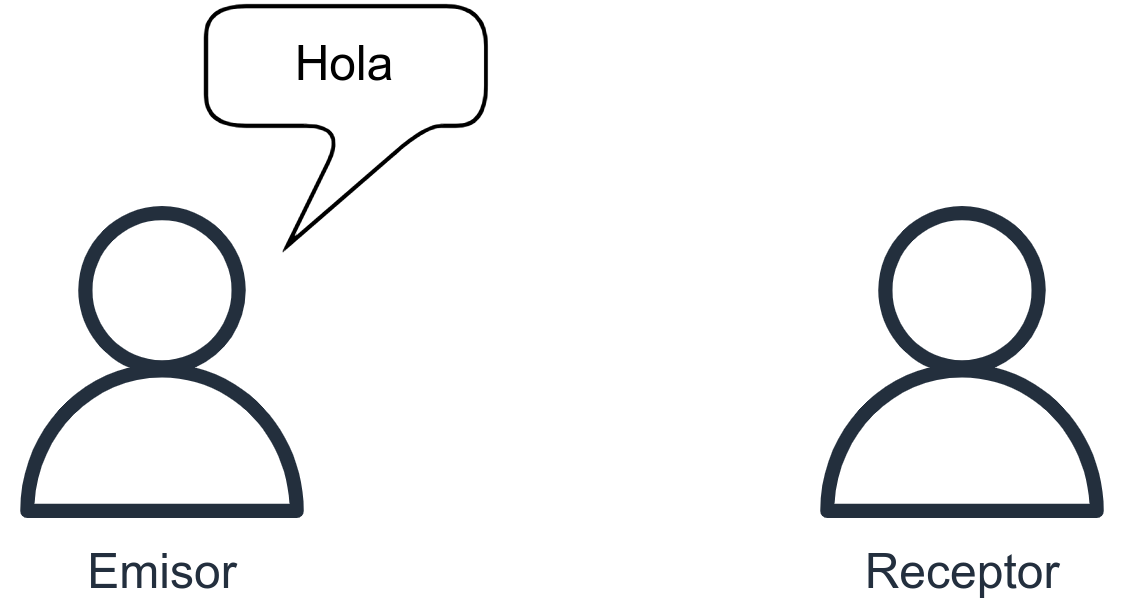
\includegraphics[width=\linewidth]{comunicacion-1.png}
    \vspace{-30pt}
\end{wrapfigure}
En este ejemplo vemos que hay dos personas, las cuales se han identificado cada una de ellas como “Emisor” y “Receptor”, y así de esta manera conocemos quién es el origen y quién el destino de la comunicación.

En este caso, el \textbf{mensaje} es “Hola”, haciendo uso del \textbf{código} conocido como “castellano”. La \textbf{señal} que se va a utilizar es la voz, ya que están hablando y el \textbf{canal} por el que se envía el mensaje es el aire.

Es un ejemplo sencillo que utilizamos cada día.

\subsubsection*{Ejemplo 2: Comunicación escrita por mensajería}

\begin{wrapfigure}{r}{0.25\linewidth}
    \centering
    \vspace{-35pt}
    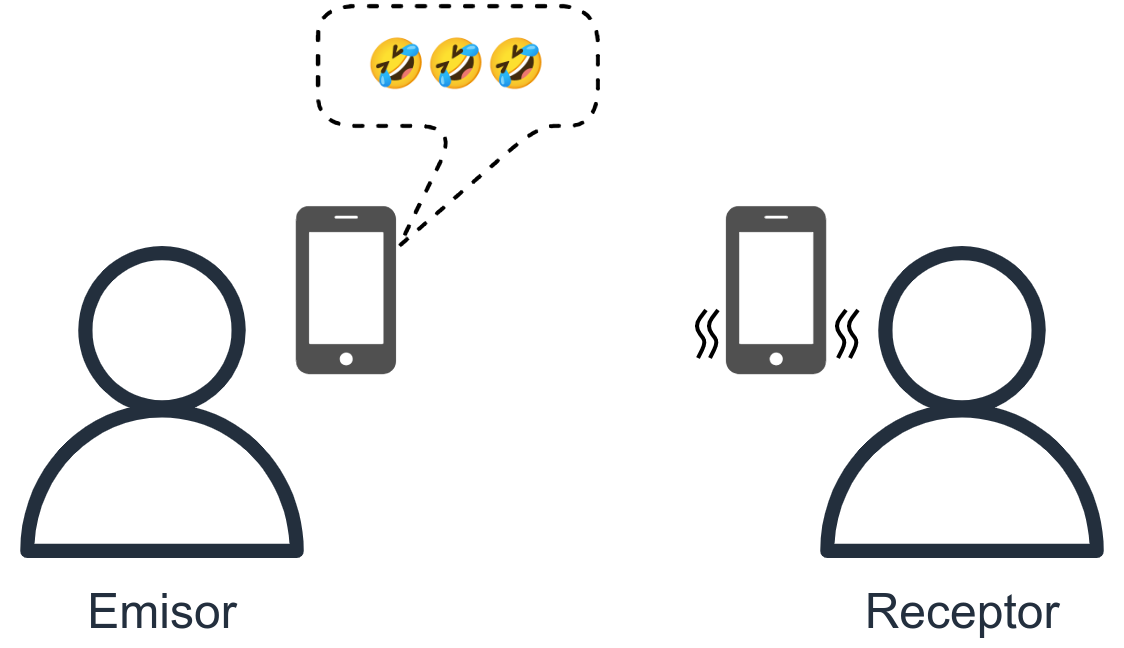
\includegraphics[width=\linewidth]{comunicacion-2.png}
    \vspace{-30pt}
\end{wrapfigure}
AL igual que en el ejemplo anterior, vemos que hay dos personas, las cuales se han identificado cada una de ellas como “Emisor” y “Receptor” pero que en este caso se van a comunicar haciendo uso de un teléfono móvil, tal como hacemos en nuestro día a día a través de una aplicación de mensajería o red social.

Teniendo en cuenta esto, en este ejemplo realmente existen dos sistemas de comunicación que están mezclados y uno está por encima del otro:

\begin{itemize}
    \item \textbf{Entre personas}: Similar al ejemplo anterior, el emisor y el receptor se están comunicando, con el mensaje compuesto por tres \href{https://es.wikipedia.org/wiki/Emoji}{emojis} que representan estar riendo. El \textbf{código} es el idioma que estén utilizando, el \textbf{canal} sería el programa utilizado y la \textbf{señal} podríamos decir que es el móvil.

    \item \textbf{Entre dispositivos}: En este caso, el emisor y receptor es el móvil de cada usuario. El mensaje es el mismo, pero convertido a un sistema digital (como el \hyperlink{binario}{binario}). El \textbf{canal} en este caso sería el aire y la \textbf{señal} es la utilizada por el móvil, por ejemplo el 5G.
\end{itemize}

Tal como se puede ver en este caso, una comunicación puede depender a su vez de otro sistema de comunicación.

\subsection{Esquema de la comunicación}
Para simplificar cómo se realiza la comunicación, podemos utilizar el siguiente esquema:

\begin{center}
    \vspace{-10pt}
    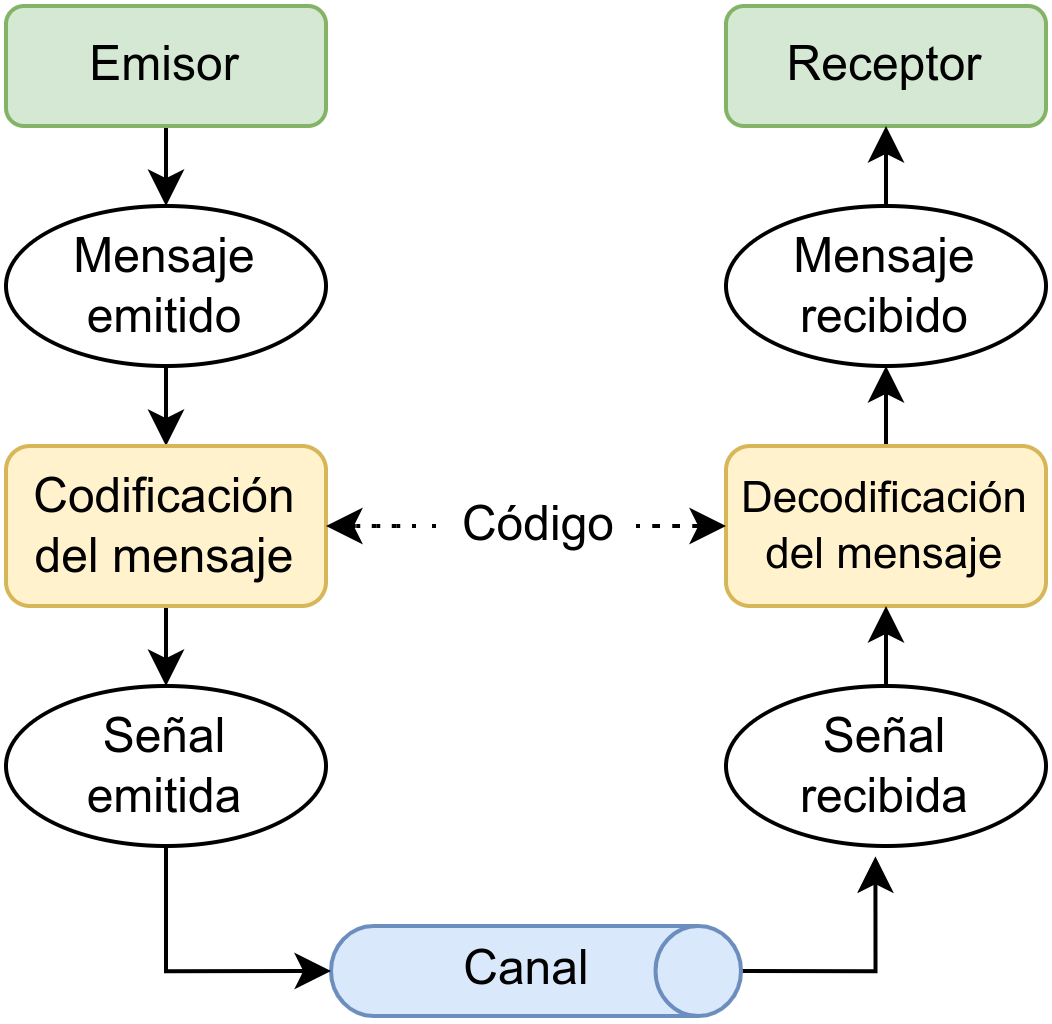
\includegraphics[width=0.6\linewidth]{comunicacion-esquema.png}
    \vspace{-10pt}
\end{center}
